\chapter{Virtualization}
\label{chap:virt}


\begin{figure*}[!ht]
  \centering
    \subfloat[Emulation ]{
      \includegraphics[width=0.3\textwidth]{figs/emulation.pdf}
      \label{fig:storage:emulation}
    }
    \hfill
    \subfloat[virtio]{
      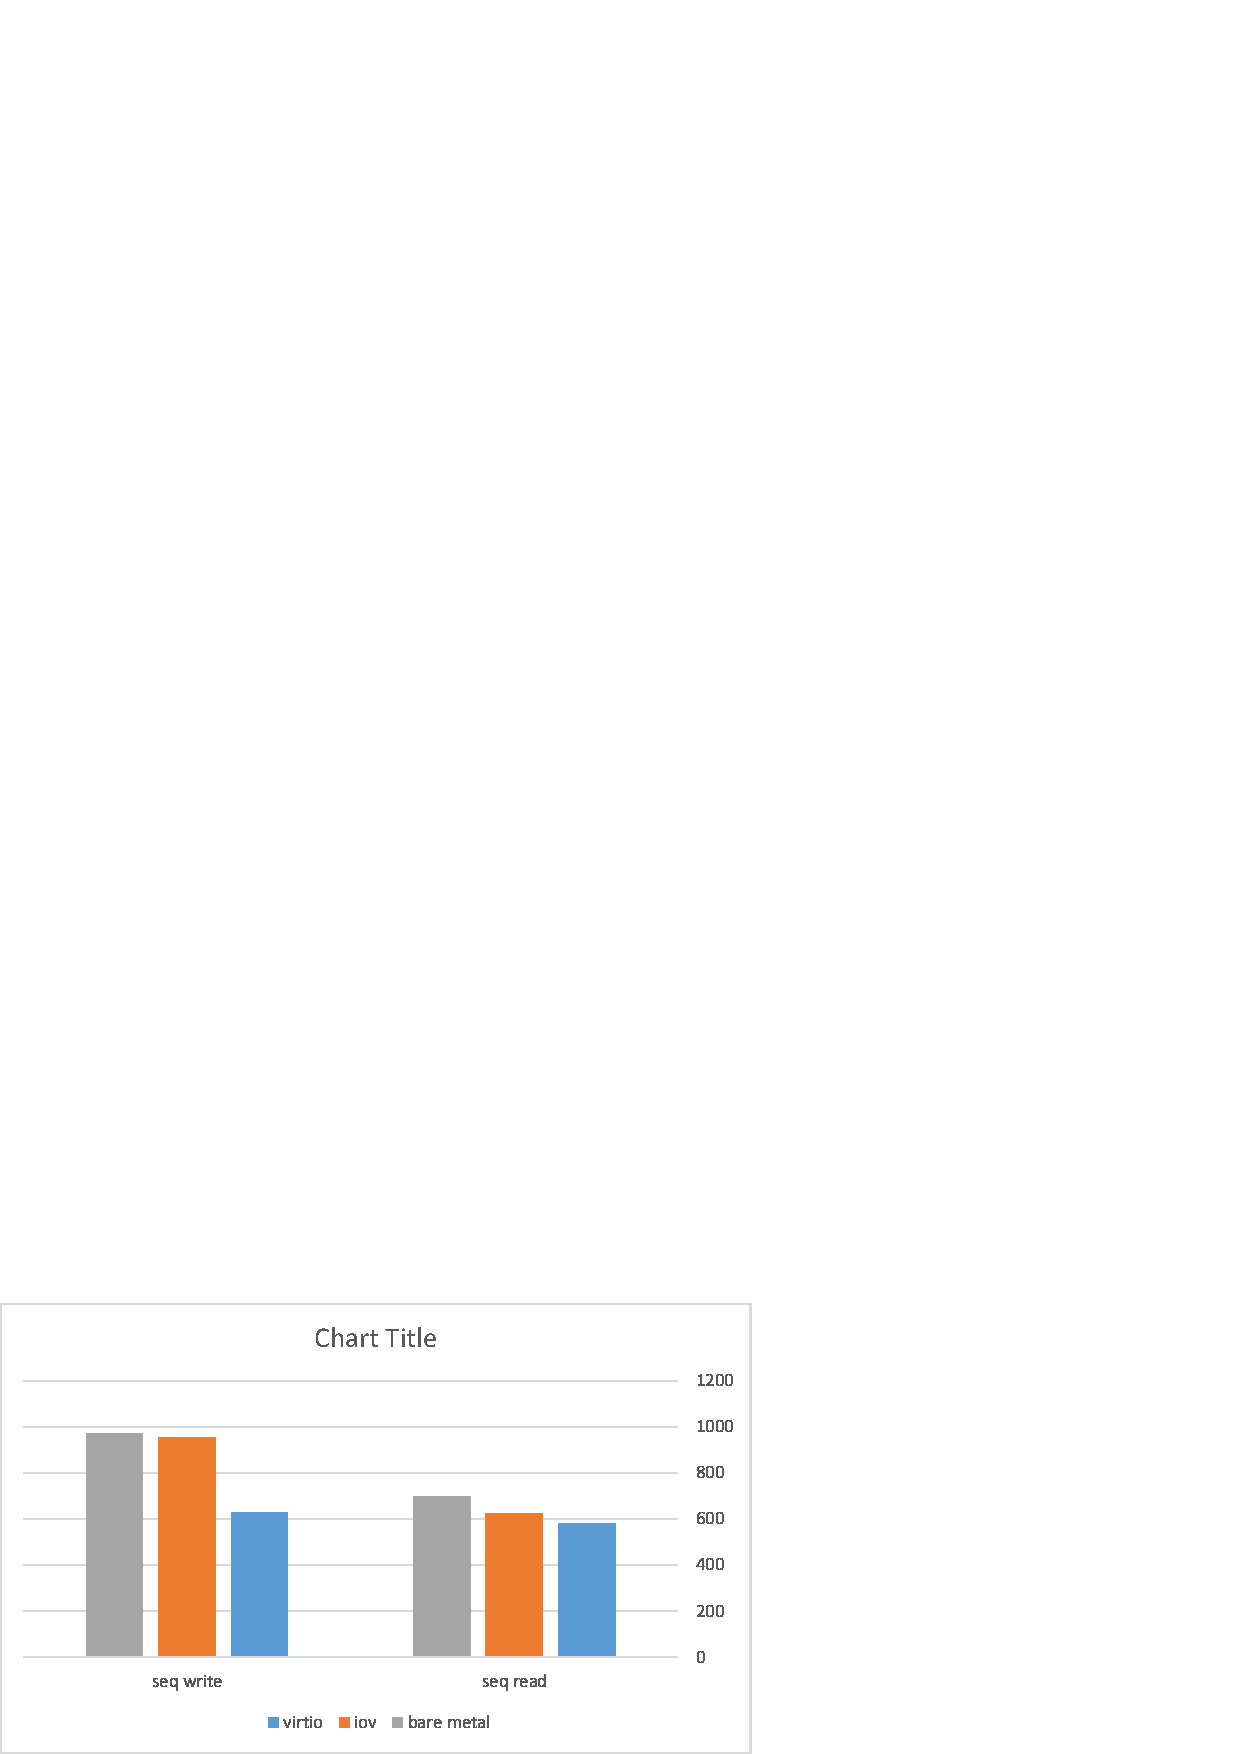
\includegraphics[width=0.3\textwidth]{figs/virtio.pdf}
      \label{fig:storage:virtio}
    }
    \hfill
    \subfloat[Direct-IO]{
      \includegraphics[width=0.3\textwidth]{figs/direct.pdf}
      \label{fig:storage:direct}
    }
    \caption{IO Virtualization techniques.
      \label{fig:storage}}
    
\end{figure*}



%%%%%%%%%%%%%%%%%%%%%%%%%%%%%%%%%%%%%%%%%%%%%%%%%%
\section{Background}
%%%%%%%%%%%%%%%%%%%%%%%%%%%%%%%%%%%%%%%%%%%%%%%%%%
\comment{cite the Xen paper some ware}
Virtualization is the act of logically dividing the system resources between different entities
running on it. Virtualization hides the physical characteristics of a computing platform from the users,
presenting instead another abstract computing platform. The software that controls the virtualization of the
system is called \emph{hypervisor} or \emph{virtual machine monitor} (VMM).

Virtualization is performed on a given hardware platform by host software (hypervisor), which creates a
simulated computer environment, a virtual machine (VM), for its guest software.
The guest software is not limited to user applications; many hosts allow the execution of complete operating
systems. The guest software executes as if it were running directly on the physical hardware, with several
notable caveats. Access to physical system resources (such as the network access, display, keyboard, and disk
storage) is generally managed at a more restrictive level than the host processor and system-memory. Guests are
often restricted from accessing specific peripheral devices, or may be limited to a subset of the device's
native capabilities, depending on the hardware access policy implemented by the virtualization host.
Virtualization often exacts performance penalties, both in resources required to run the hypervisor,
and as well as in reduced performance on the virtual machine compared to running native on the physical machine.


%%%%%%%%%%%%%%%%%%%%%%%%%%%%%%%%%%%%%%%%%%%%%%%%%%
\section{Virtualization Aspects}
%%%%%%%%%%%%%%%%%%%%%%%%%%%%%%%%%%%%%%%%%%%%%%%%%%
There are 3 main resources that the hypervisor needs to virtualize: the CPU, Memory and I/O devices.

\paragraph {CPU}
A common implementation of CPU virtualizing is \emph{Trap-and-Emulate}. When using this technique,
the guest code (OS or user application) may run directly on the CPU and only when an unprivileged command is
executed, the CPU will issue a trap to the hypervisor which will handle the guest command.

\paragraph {Memory}
A guest OS has no control over the hosts physical memory (just like any other process). The page tables set by the
guest OS keep the translation from \emph{guest virtaul address} to \emph{guest physical address}. Modern
processors use \emph{Extended Page Tables} (EPT) technology. This technology enables the \emph{MMU} to do a
double translation: First it translates the \emph{guest virtaul address} to \emph{guest physical address} using the page tables set by the guest OS. Then it translates the \emph{guest physical address} to \emph{host physical address} using the page tables set by the hypervisor.
\comment{Should i talk about shadow page tables?}

\paragraph {I/O devices}
Its the hypervisor responsibility to share an I/O device between virtual machines. While sharing a device, isolation must be enforced so that one VM cannot access other VMs' resources on an I/O device.  

Figure~\ref{fig:storage} illustrates the three most common methods by which hypervisors virtualize storage devices (We discuss storage devices, but the same technologies work for any I/O device ):

\begin{enumerate}
\item
  \emph{Full device emulation}~\cite{sugerman2001virtualizing} (Figure~\ref{fig:storage:emulation})\quad 
  In this method, the host emulates a known device that the guest already has a driver for. The host traps device accesses by the VM and converts them to operations on real hardware. The emulated device is represented as a file on the host filesystem, and whenever the guest tries to access a virtual LBA on the device, the host converts the virtual LBA to an offset in the file.

\item
  \emph{Paravirtualization}~\cite{barham2003xen,russell2008virtio} (Figure~\ref{fig:storage:virtio})\quad
  This method, commonly referred to as virtio after its Linux implementation, eliminates the need for the hypervisor to emulate a complete physical device and enables the guest VM to directly request a virtual LBA from the hypervisor, thereby improving performance. This is the most common storage virtualization method used in modern hypervisors.

\item
  \emph{Direct device assignment}~\cite{raj2007high} (Figure~\ref{fig:storage:direct})\quad
  This method allows the guest VM to directly interact with the physical device without hypervisor mediation. Consequently, it delivers the best storage performance to the VM. However, since storage devices do not enforce isolation among clients, it does not allow multiple VMs to share a physical device.
\end{enumerate}



